\documentclass[11pt,a4paper]{report}
\usepackage[utf8]{inputenc}
\usepackage[portuguese]{babel}
\usepackage[T1]{fontenc}
\usepackage{amsmath}
\usepackage{amsfonts}
\usepackage{amssymb}
\usepackage{graphicx}
\author{Altair Ramos}
\begin{document}

\chapter*{Ananke}
\section*{Ascensão Reta}
\begin{figure}[h]
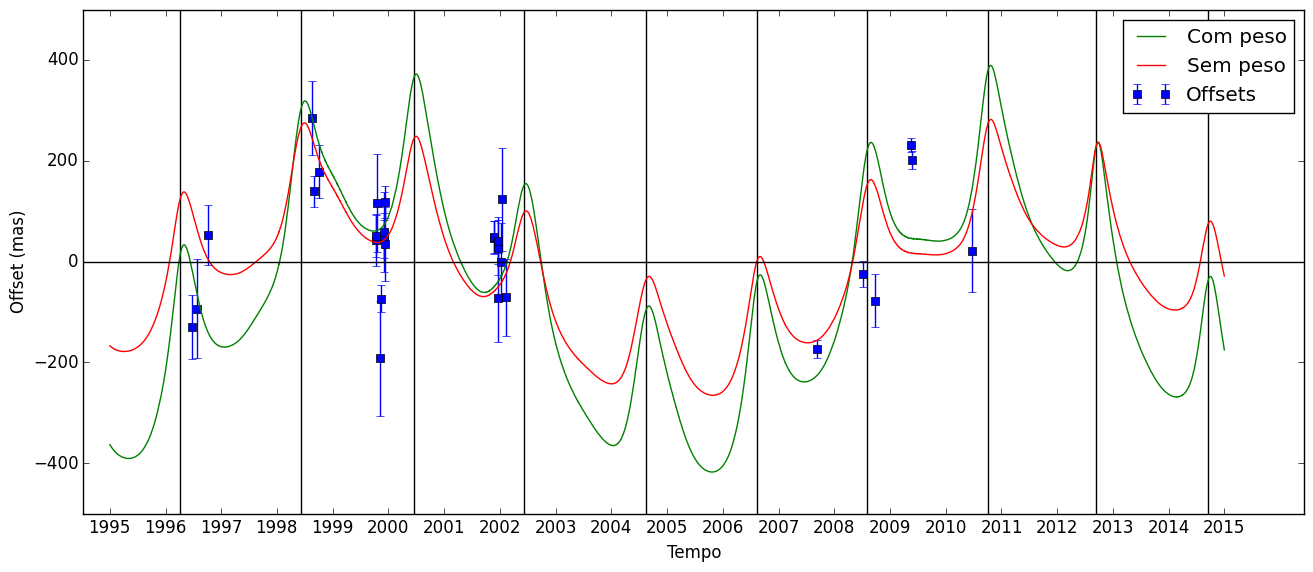
\includegraphics[scale=0.35]{Ananke/RA.png} 
\end{figure}

\indent Resultados do ajuste com peso:\\
p[0]: 246 $\pm$ 39\\
p[1]: 10.8 $\pm$ 0.5\\
p[2]: 0.09 $\pm$ 0.15\\
p[3]: 60 $\pm$ 29\\
p[4]: 152 $\pm$ 37\\
p[5]: -20 $\pm$ 37\\
Residuos: 571 mas\\

Resultados do ajuste sem peso:\\
p[0]: 160 $\pm$ 43\\
p[1]: 12.0 $\pm$ 0.9\\
p[2]: 0.4 $\pm$ 0.1\\
p[3]: 44 $\pm$ 39\\
p[4]: 111 $\pm$ 32\\
p[5]: 5 $\pm$ 37\\
Residuos: 451 mas\\

\section*{Declinação}

\begin{figure}[h]
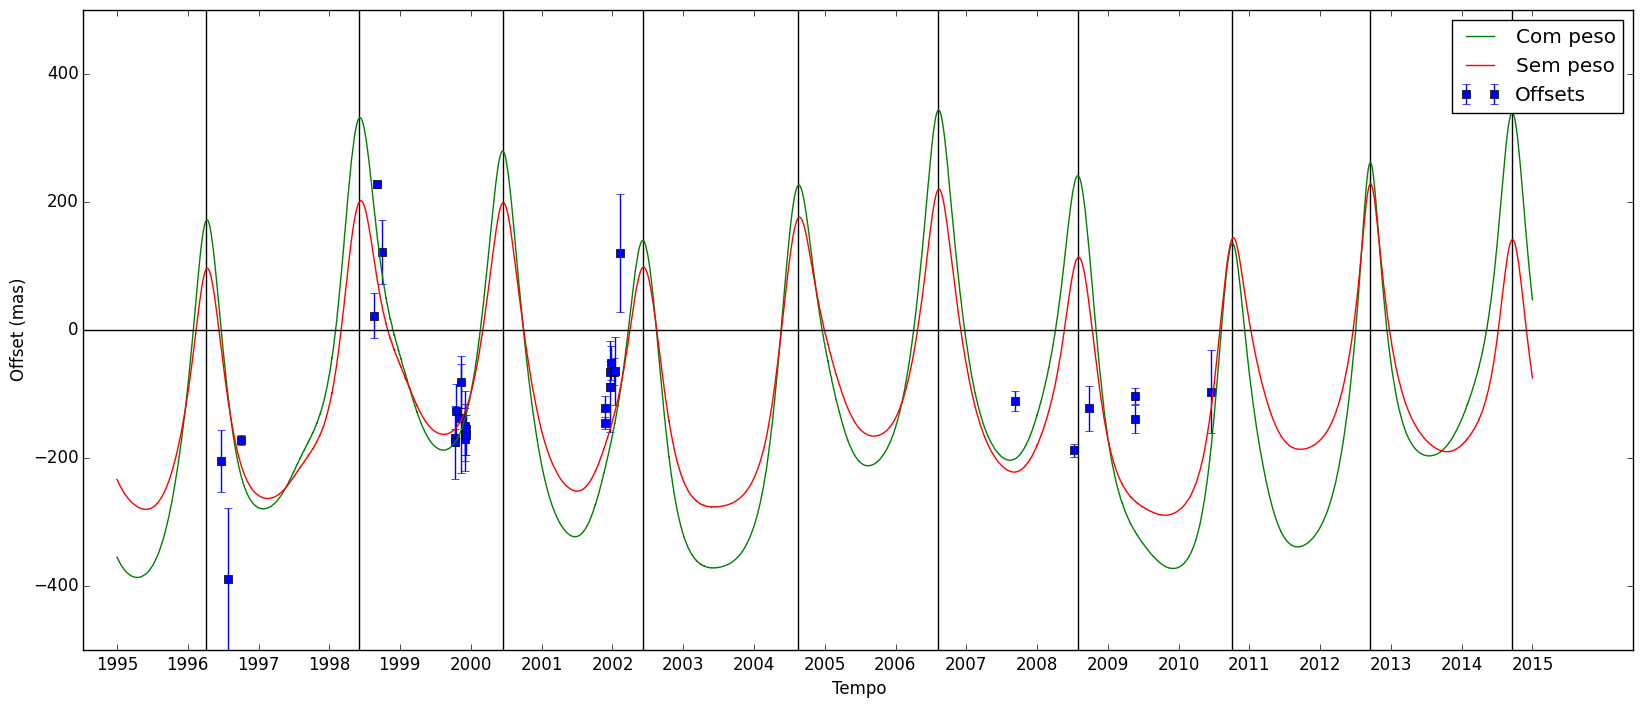
\includegraphics[scale=0.35]{Ananke/DEC.png} 
\end{figure}

\chapter*{Carme}
\section*{Ascensão Reta}
\begin{figure}[h]
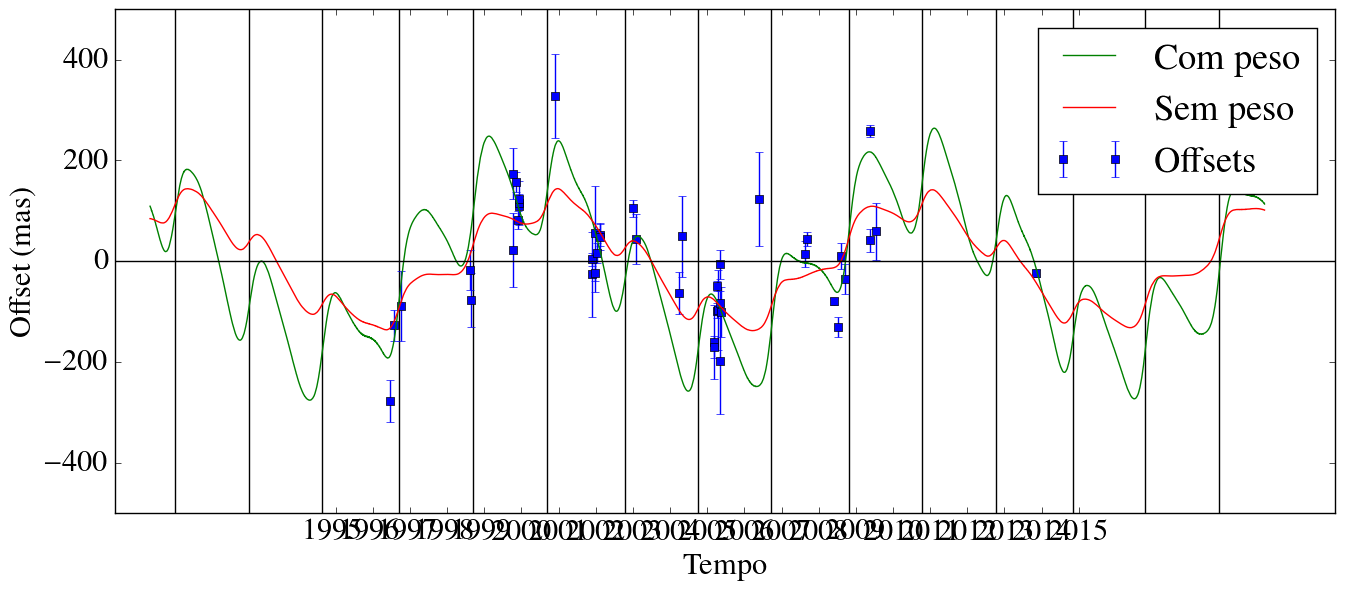
\includegraphics[scale=0.35]{Carme/RA.png} 
\end{figure}

\section*{Declinação}

\begin{figure}[h]
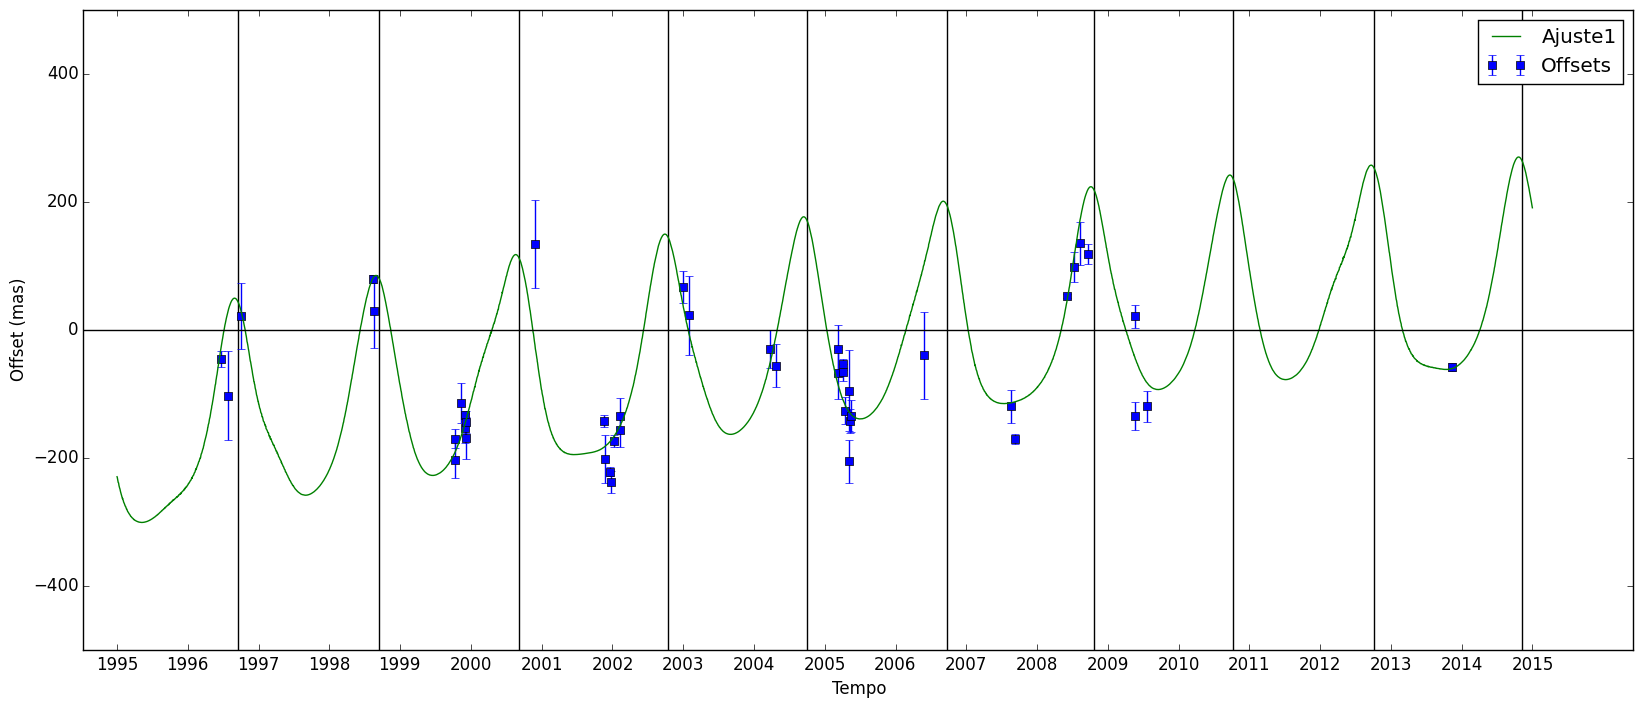
\includegraphics[scale=0.35]{Carme/DEC.png} 
\end{figure}

\chapter*{Elara}
\section*{Ascensão Reta}

\begin{figure}[h]
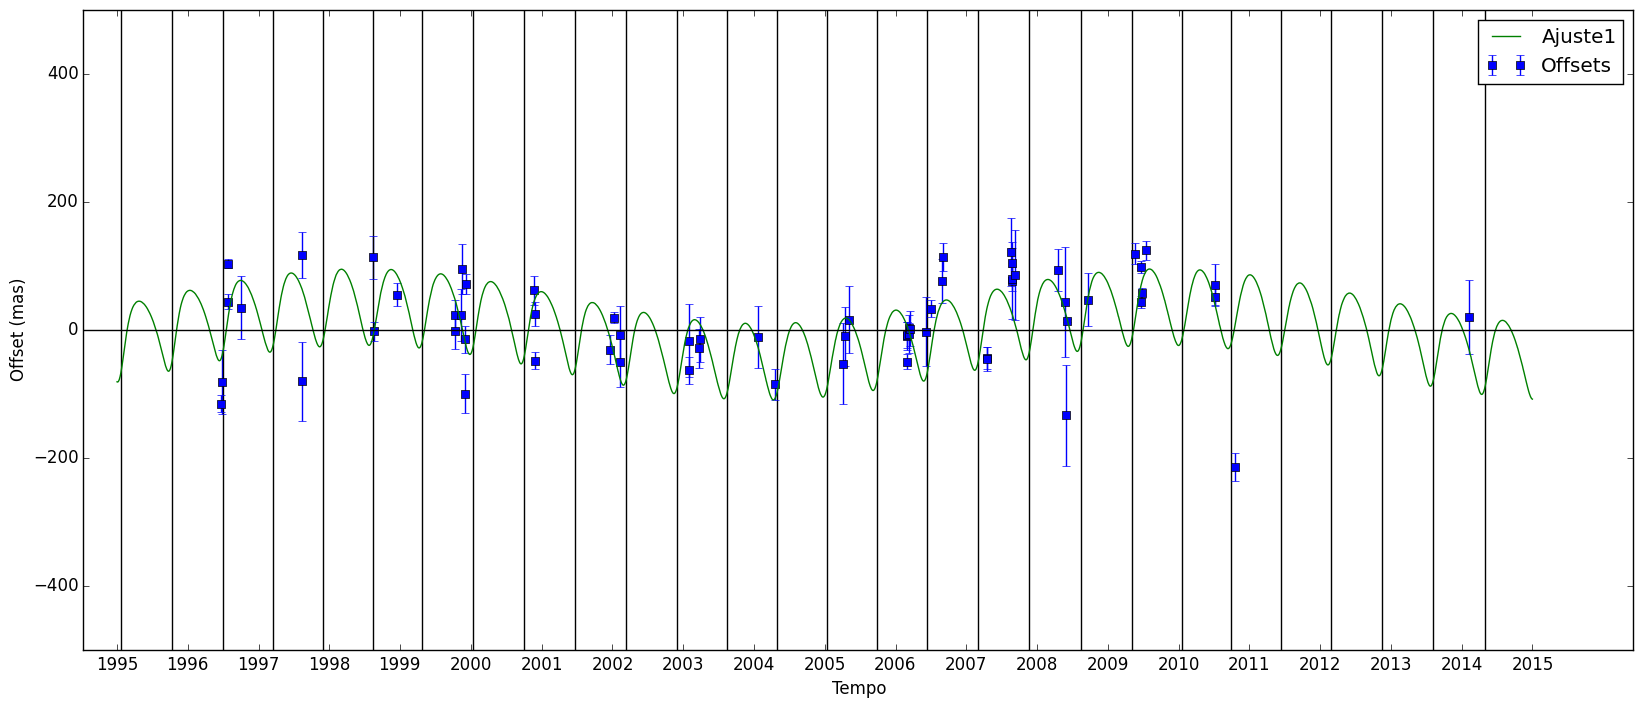
\includegraphics[scale=0.35]{Elara/RA.png} 
\end{figure}

\section*{Declinação}

\begin{figure}[h]
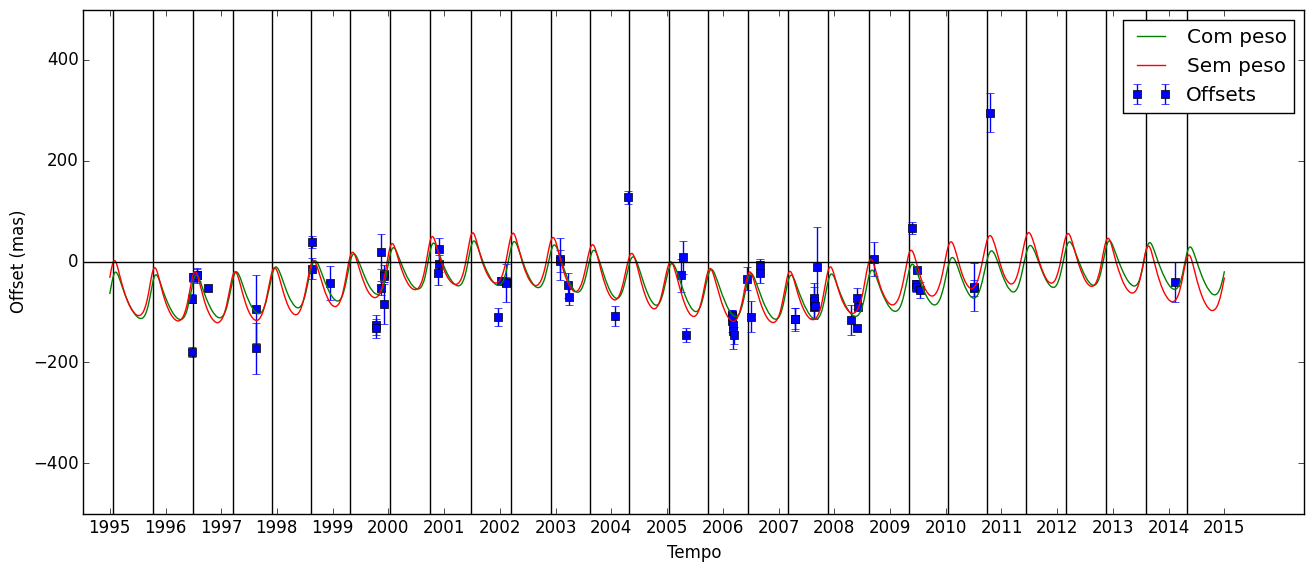
\includegraphics[scale=0.35]{Elara/DEC.png} 
\end{figure}

\chapter*{Himalia}
\section*{Ascensão Reta}

\begin{figure}[h]
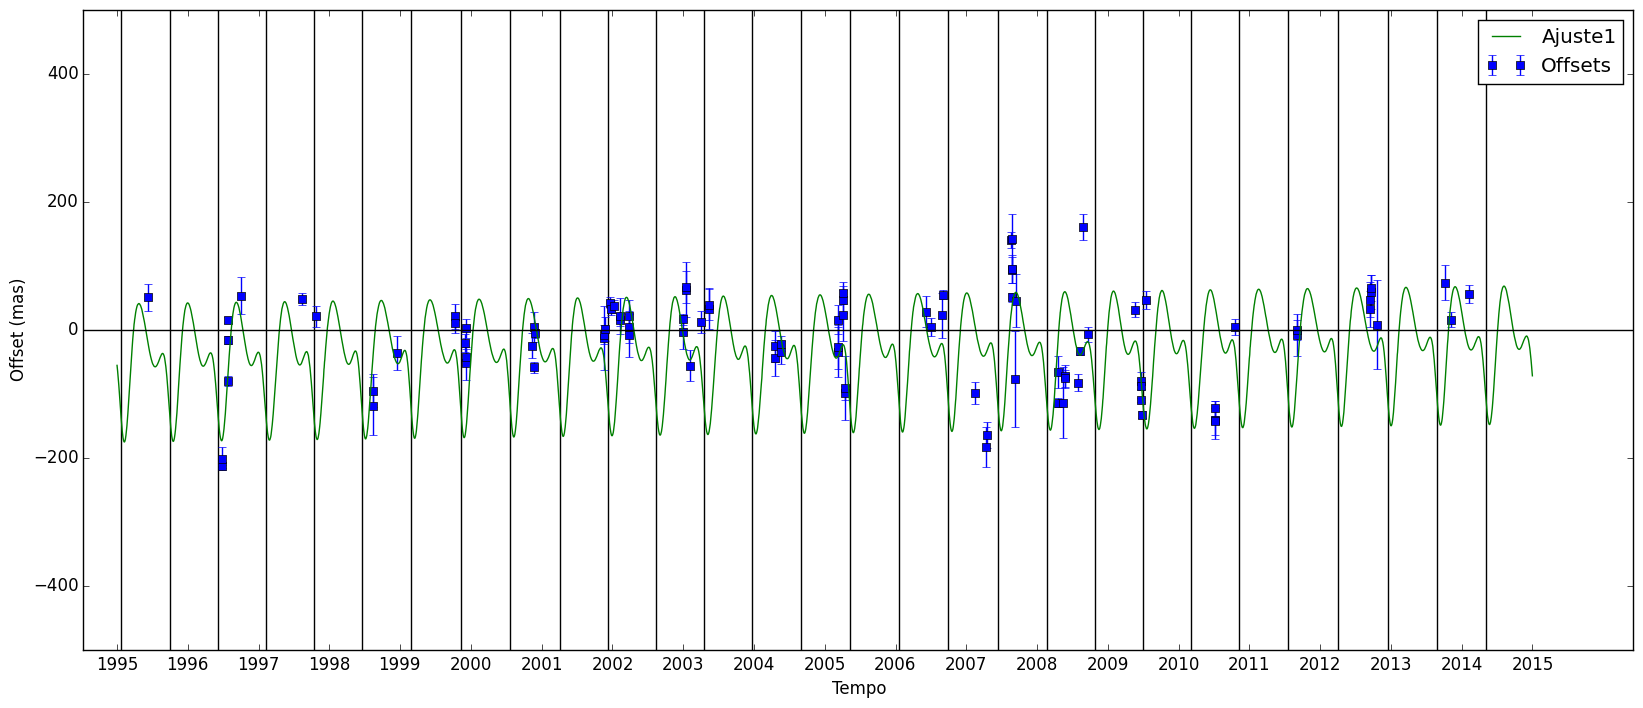
\includegraphics[scale=0.35]{Himalia/RA.png} 
\end{figure}

\section*{Declinação}

\begin{figure}[h]
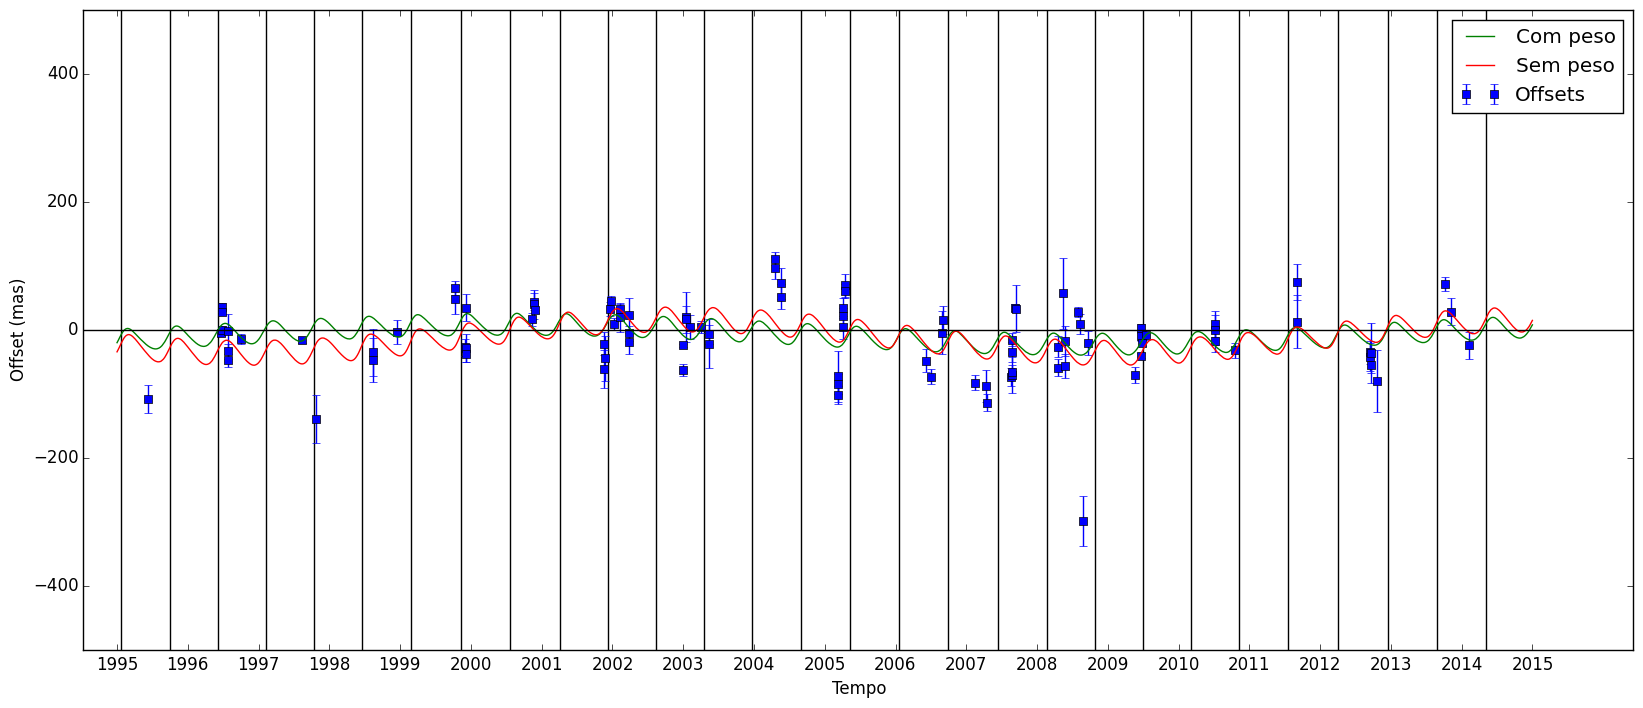
\includegraphics[scale=0.35]{Himalia/DEC.png} 
\end{figure}

\chapter*{Lysithea}
\section*{Ascensão Reta}

\begin{figure}[h]
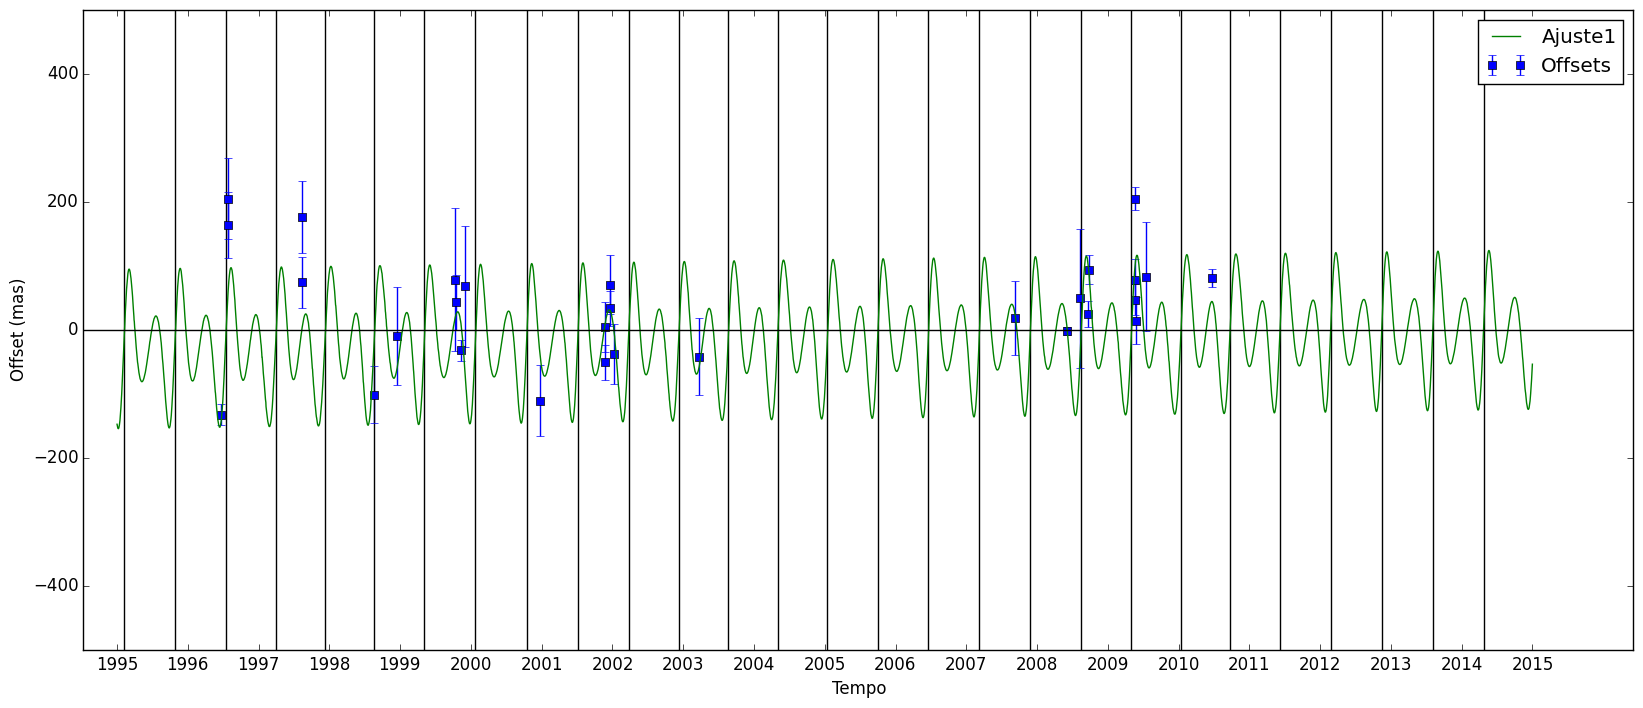
\includegraphics[scale=0.35]{Lysithea/RA.png} 
\end{figure}

\section*{Declinação}

\begin{figure}[h]
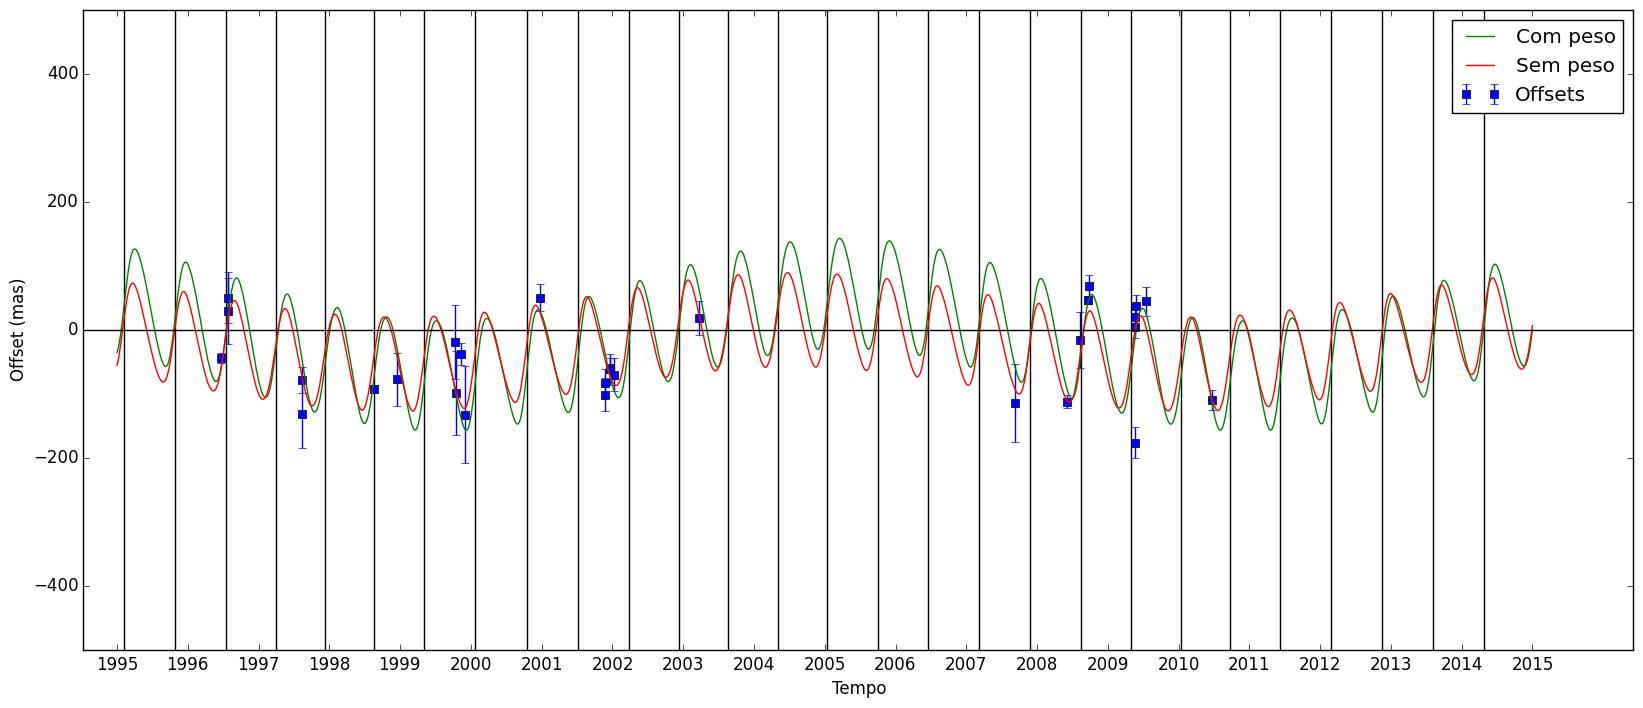
\includegraphics[scale=0.35]{Lysithea/DEC.png} 
\end{figure}

\chapter*{Sinope}
\section*{Ascensão Reta}

\begin{figure}[h]
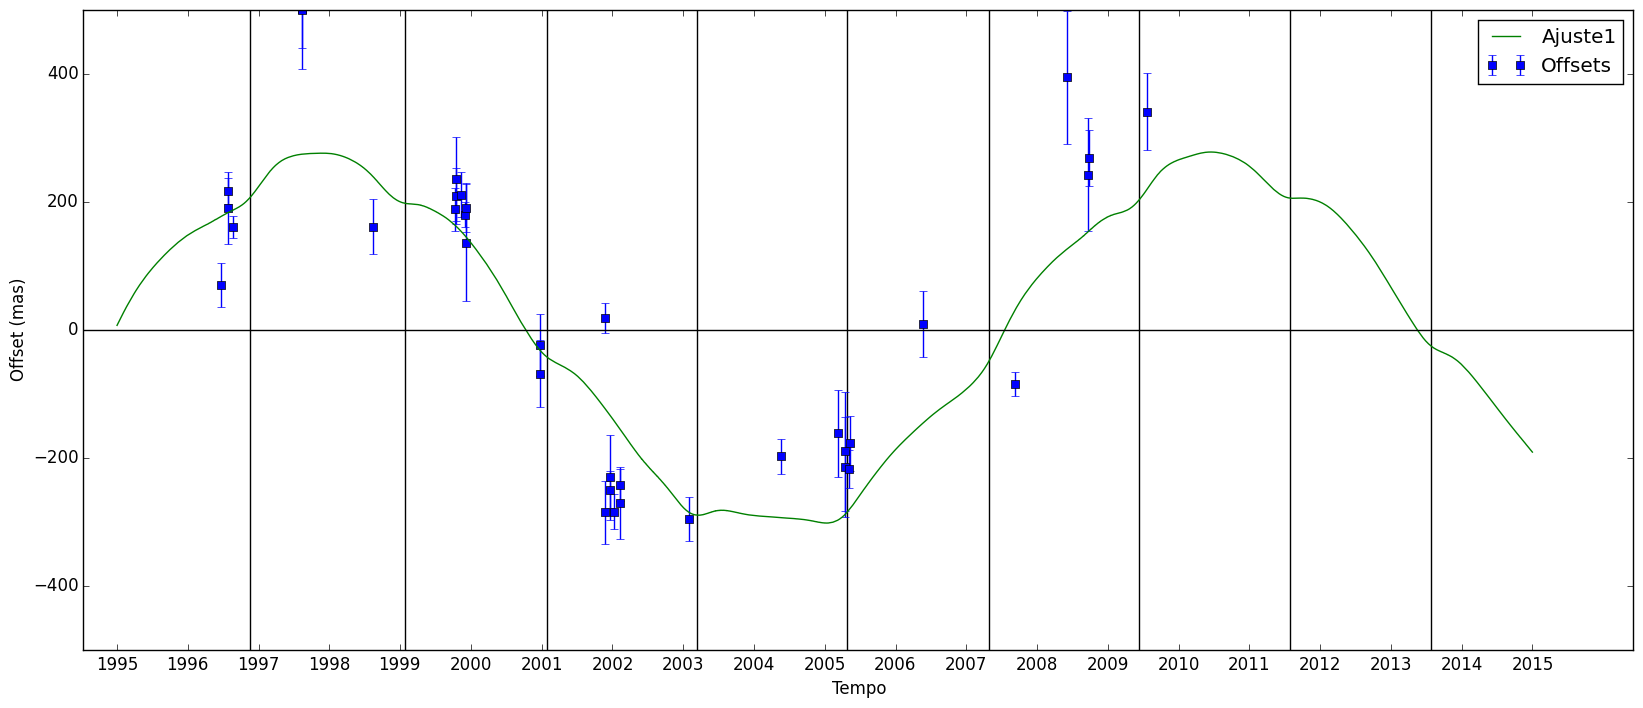
\includegraphics[scale=0.35]{Sinope/RA.png} 
\end{figure}

\section*{Declinação}

\begin{figure}[h]
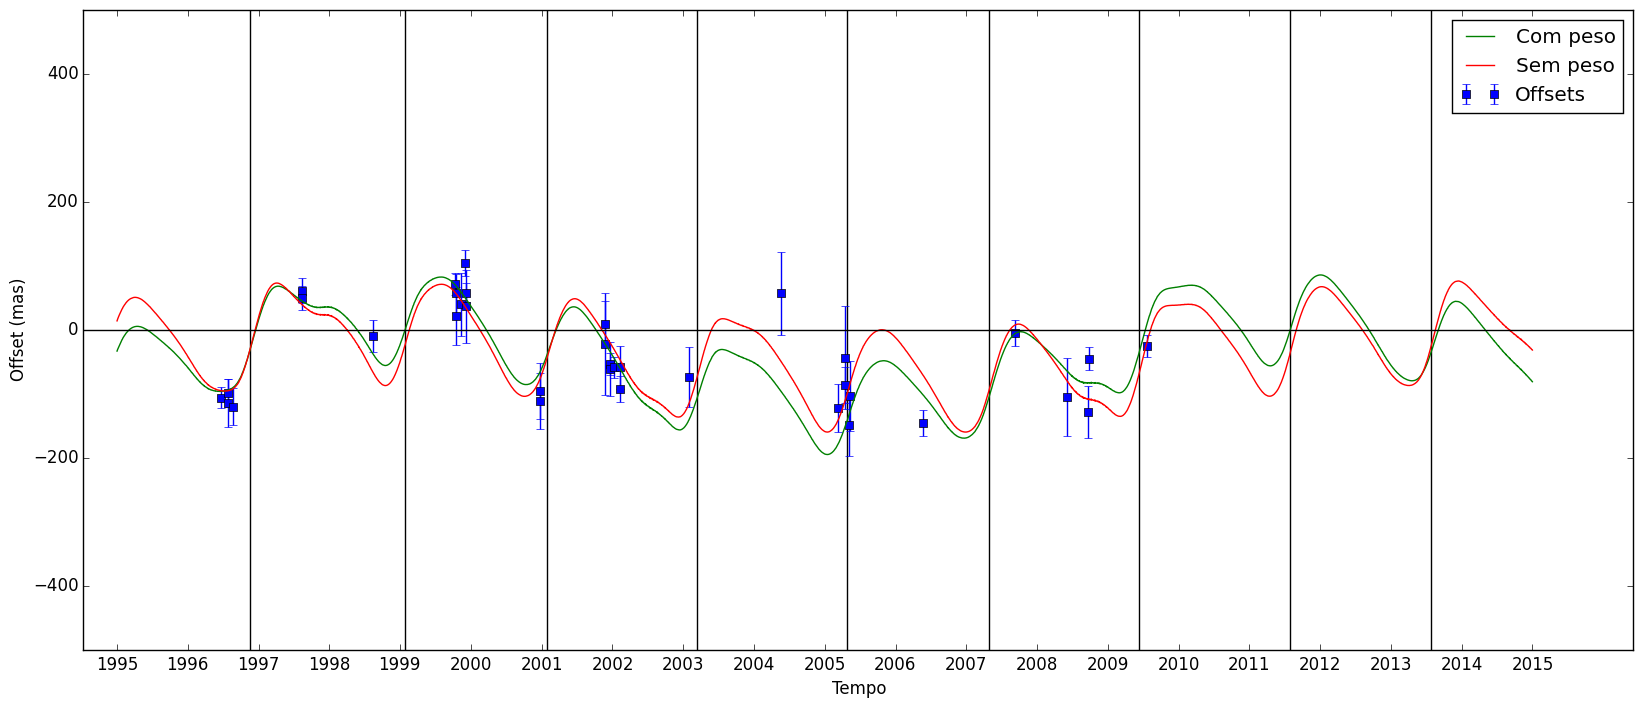
\includegraphics[scale=0.35]{Sinope/DEC.png} 
\end{figure}

\chapter*{Pasiphae}
\section*{Ascensão Reta}

\begin{figure}[h]
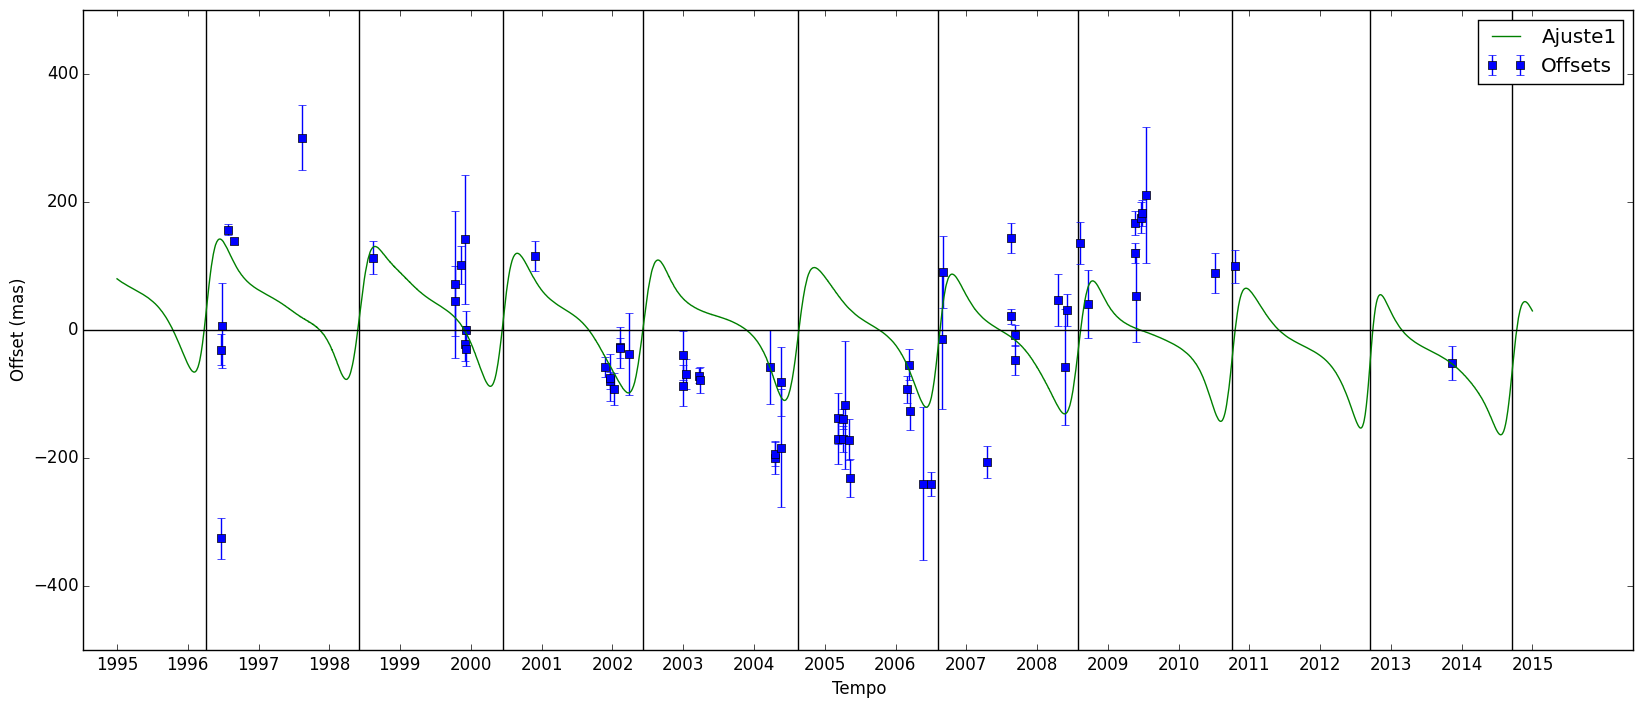
\includegraphics[scale=0.35]{Pasiphae/RA.png} 
\end{figure}

\section*{Declinação}

\begin{figure}[h]
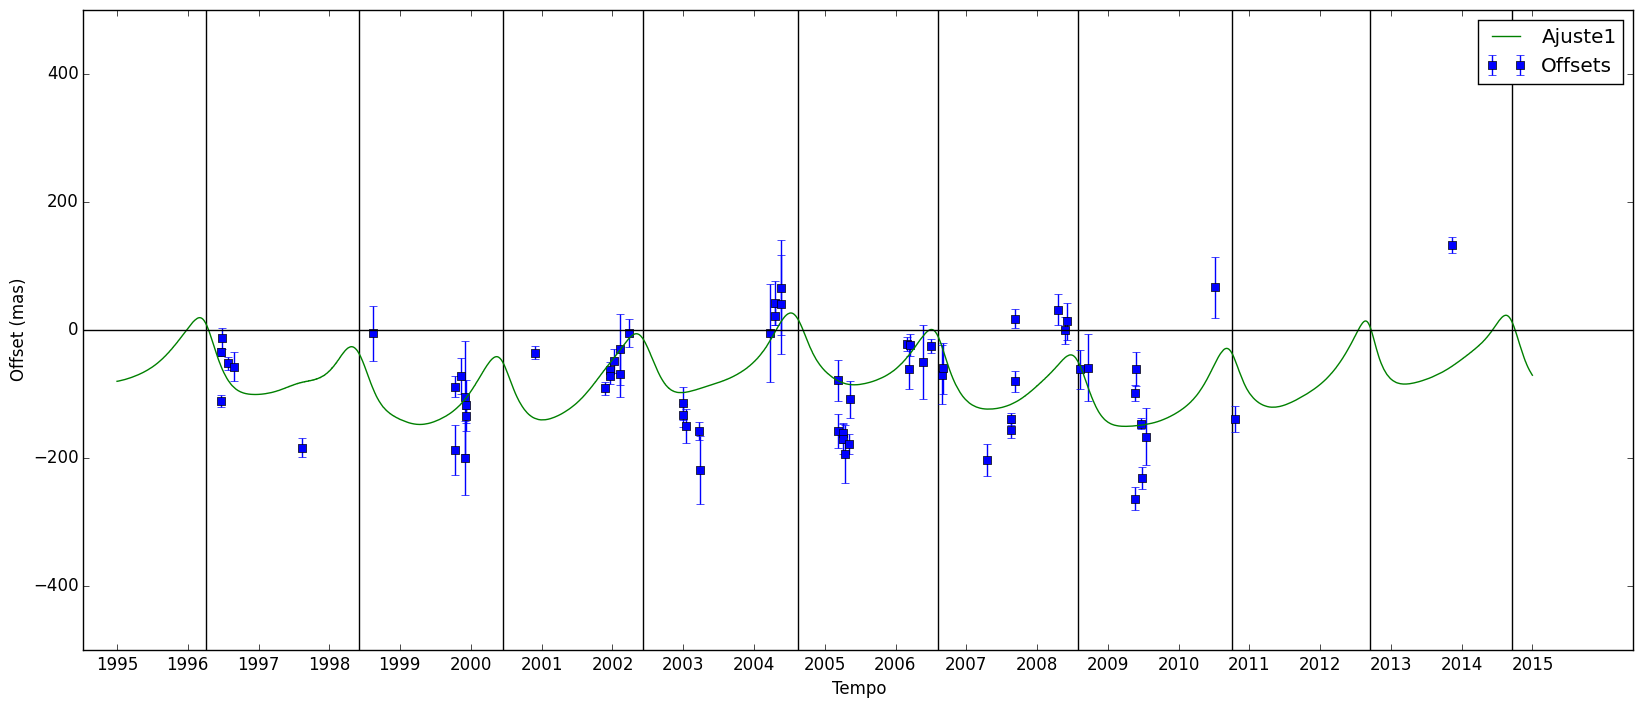
\includegraphics[scale=0.35]{Pasiphae/DEC.png} 
\end{figure}

\chapter*{Phoebe}
\section*{Ascensão Reta}

\begin{figure}[h]
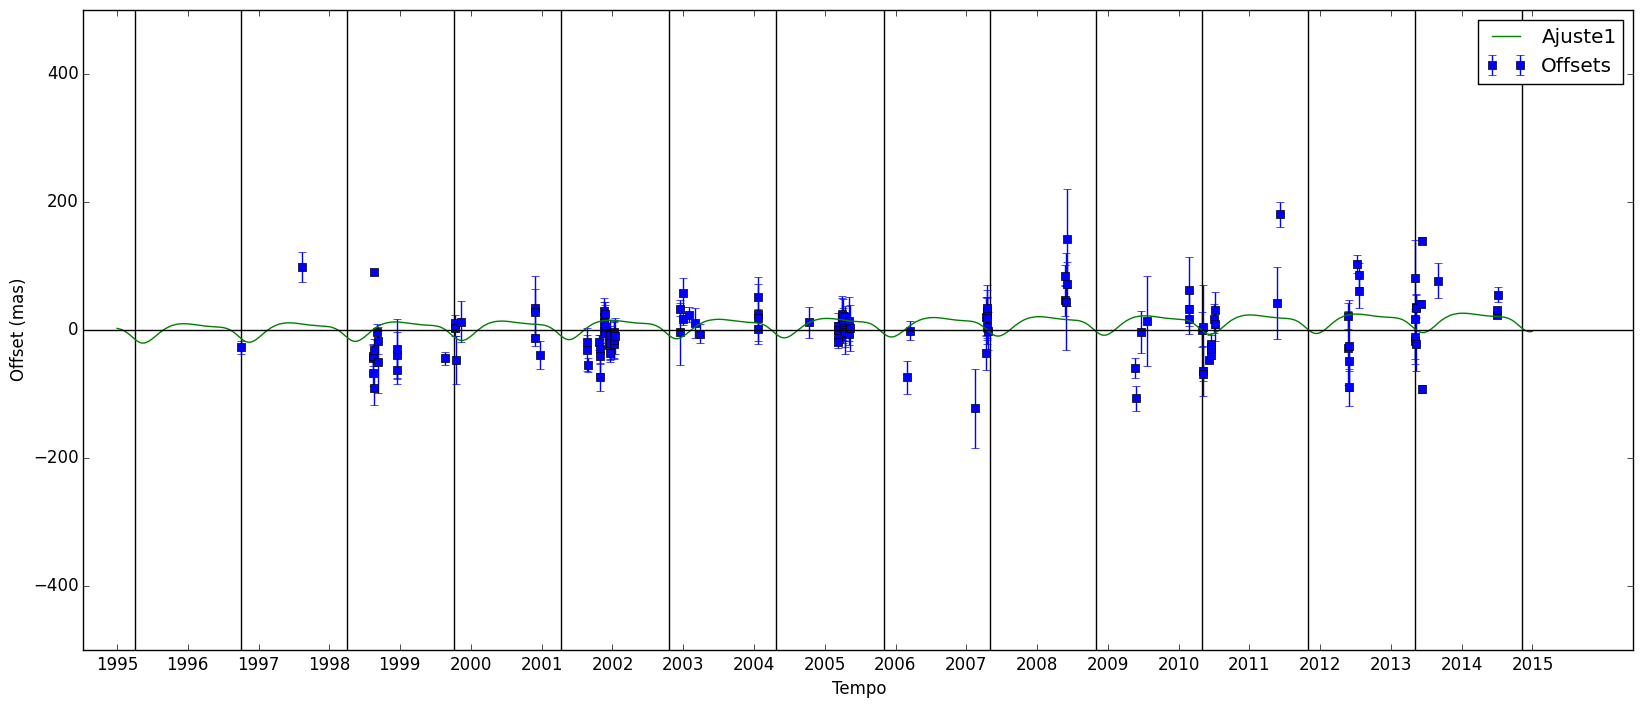
\includegraphics[scale=0.35]{Phoebe/RA.png} 
\end{figure}

\section*{Declinação}

\begin{figure}[h]
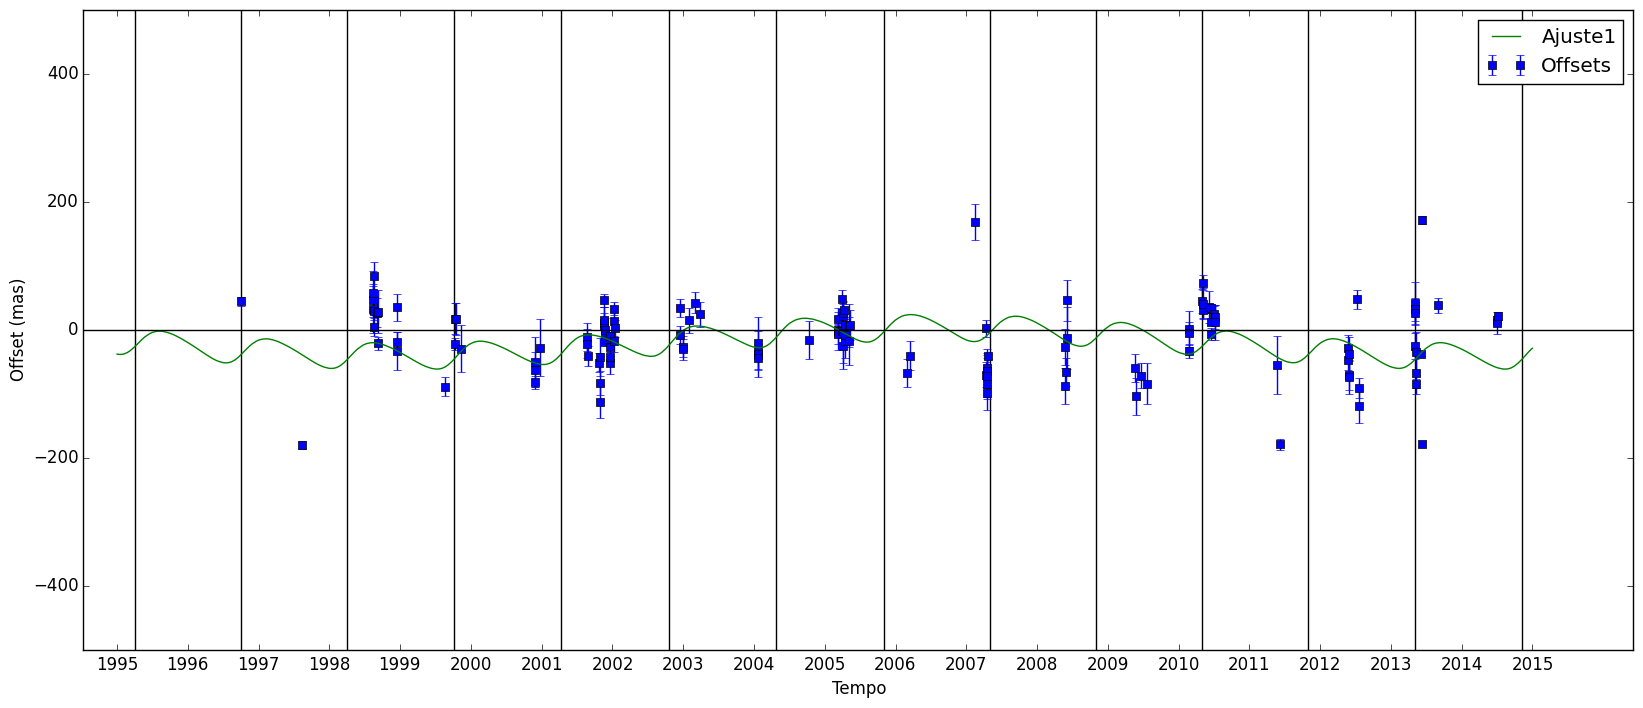
\includegraphics[scale=0.35]{Phoebe/DEC.png} 
\end{figure}

\chapter*{Nereida}
\section*{Ascensão Reta}

\begin{figure}[h]
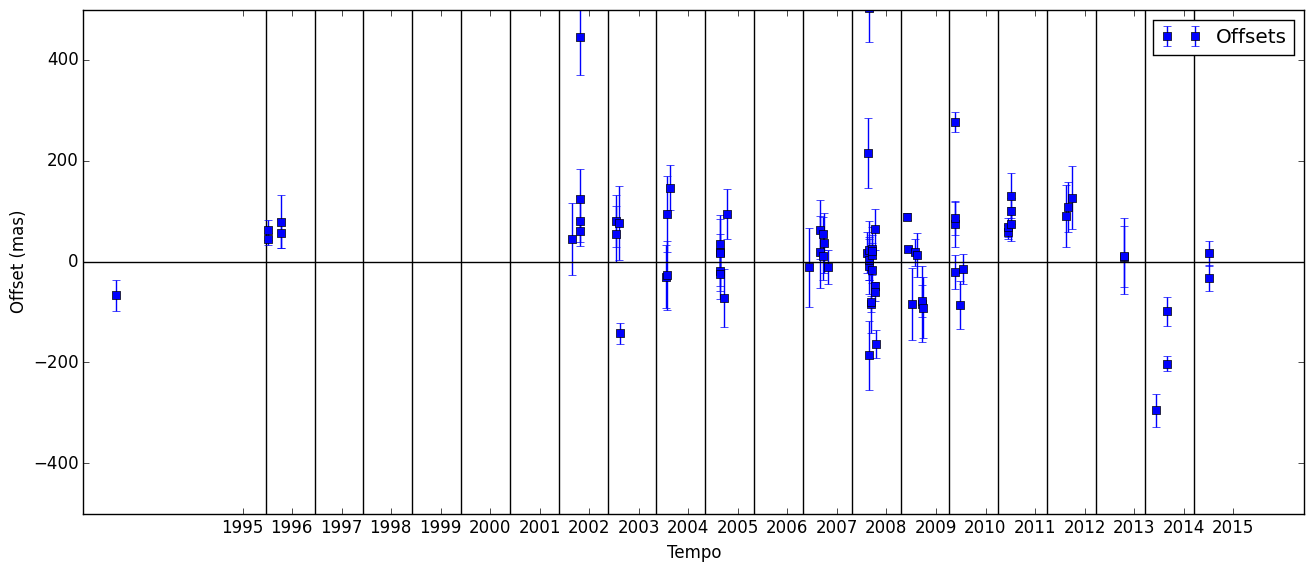
\includegraphics[scale=0.35]{Nereida/RA.png} 
\end{figure}

\section*{Declinação}

\begin{figure}[h]
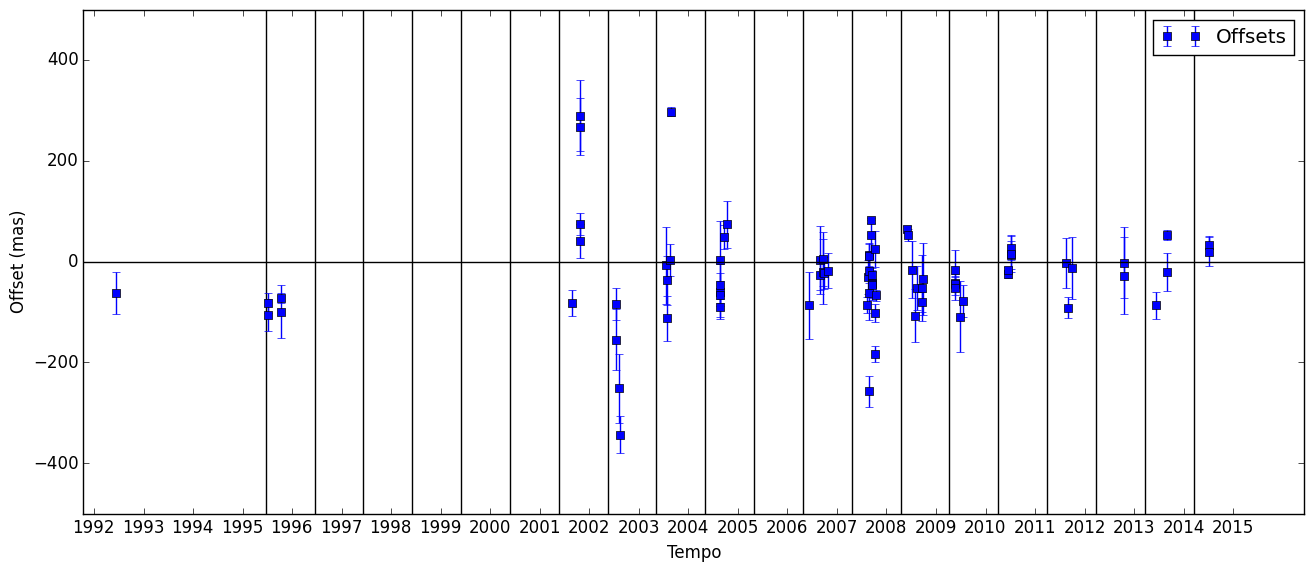
\includegraphics[scale=0.35]{Nereida/DEC.png} 
\end{figure}

\end{document}